\documentclass[17pt]{beamer}
%\documentclass[handout]{beamer} %Makes Handouts
\usetheme{Singapore} %Gray with fade at top
\useoutertheme[subsection=false]{miniframes} %Supppress subsection in header
\useinnertheme{rectangles} %Itemize/Enumerate boxes
\usecolortheme{seagull} %Color theme
\usecolortheme{rose} %Inner color theme

\definecolor{light-gray}{gray}{0.75}
\definecolor{dark-gray}{gray}{0.55}
\setbeamercolor{item}{fg=light-gray}
\setbeamercolor{enumerate item}{fg=dark-gray}

\setbeamertemplate{navigation symbols}{}
\setbeamertemplate{mini frames}{}
%\setbeamercovered{dynamics}
\setbeamerfont*{title}{size=\Large,series=\bfseries}
\setbeamerfont{footnote}{size=\tiny}

%\setbeameroption{notes on second screen} %Dual-Screen Notes
%\setbeameroption{show only notes} %Notes Output

\setbeamertemplate{frametitle}{\vspace{.5em}\bfseries\insertframetitle}
\newcommand{\heading}[1]{\noindent \textbf{#1}\\ \vspace{1em}}
\newcommand{\questions}{\frame{{\large Questions?}}}

\usepackage{bbding,color,multirow,times,ccaption,tabularx,graphicx,verbatim,booktabs}
\usepackage{colortbl} %Table overlays
\usepackage[english]{babel}
\usepackage[latin1]{inputenc}
\usepackage[T1]{fontenc}
\usepackage{lmodern}
\usepackage{alltt}

\usepackage{tikz}
\usetikzlibrary{shapes,arrows,decorations.pathreplacing,calc}


\author[]{Thomas J. Leeper}
\institute{
  Government Department\\London School of Economics and Political Science
}


\title{Session III\\External Validity}

\date[]{}

\begin{document}

\frame{\titlepage}

\frame{

\frametitle{Reminder: Friday}

If you're interested in presenting an idea for a survey experiment on Friday, let me know in person or via email.

}


\frame{

\frametitle{Review}

What techniques can we use to assess whether a treatment manipulated what we wanted it to and did not manipulate what we didn't want it to?

}

\frame{

\frametitle{Review}

What are some of the available paradigms for implementing a survey experiment?

}

\frame{

\frametitle{Review}

What is an experimental protocol document and why is it useful?

}



\frame{\tableofcontents}

\section[External Validity]{External Validity of a Sample}
\frame{\tableofcontents[currentsection]}

\frame{

\frametitle{Think--Pair--Share}

Consider the following question:

What makes an experiment (or any research study) generalizable? What does it mean for a study's results to ``generalize''?

\begin{enumerate}
\item Write or think to yourself for 90 seconds
\item Then, discuss with the person next to you
\end{enumerate}

}


\frame{
\frametitle{{\normalsize ``The Gold Standard''}}

\small
\textit{a population-based experiment uses survey sampling methods to produce a collection of experimental subjects that is representative of the target population of interest for a particular theory \dots the population represented by the sample should be representative of the population to which the researcher intends to extend his or her findings. In population-based experiments, experimental subjects are randomly assigned to conditions by the researcher}\\

\vspace{0.5em}
{\footnotesize p2. from Mutz, Diana. 2011. \textit{Population-Based Survey Experiments}. Princeton University Press.\par}

}


\frame{
	\frametitle{Surveys Start with an Inference Population}
	
	\small
	\begin{itemize}\itemsep0.25em
		\item We want to speak to a population
		\item But what population is it?
			\begin{itemize}
			\item<2-> A national population?
			\item<3-> Adults in Western, industrialized democracies?
			\item<4-> All human beings?
			\end{itemize}
		\item<5-> This is rarely specified, but is important when we think about whether a sample is appropriate
	\end{itemize}
}



\frame{
	\frametitle{A Hypothetical Census}

	\begin{itemize}\itemsep1em
		\item Advantages
			\begin{itemize}
				\item<2-> Perfectly representative
				\item<2-> Sample statistics are population parameters
			\end{itemize}
		\item Disadvantages
			\begin{itemize}
				\item<3-> Costs
				\item<3-> Feasibility
				\item<3-> Need
			\end{itemize}		
	\end{itemize}
}


\subsection{Design-based}
\frame{\tableofcontents[currentsection, currentsubsection]}

\frame{

\frametitle{{\normalsize Sampling Considerations\dots}}

\small

\begin{itemize}\itemsep0.25em
\item Design-based survey samples all work from the premise of each unit having a \textit{known, non-zero} probability of being sampled
	\begin{itemize}\footnotesize
	\item SRS is representative per se
	\item Non-self-weighting samples representative when weighted
	\end{itemize}
\item<2-> Random sampling ensures that samples are, \textit{in expectation}, representative of the population \textit{in all respects}
	\begin{itemize}\footnotesize
	\item Demographics
	\item Covariances
	\item Potential outcomes
	\end{itemize}
\end{itemize}
}


\frame{}

\begin{frame}[plain]{}
\frametitle{Representativeness}

\vspace{0.25em}

What does it mean for a sample to be representative?

\begin{itemize}\small
	\item<2-> Census?
	\item<3-> Probability-based sampling?
	\item<4-> Quota fulfillment?
	\item<5-> Others?
\end{itemize}

\onslide<6->{Which of these matter?}
\end{frame}

% what kinds of representativeness do we care about?



\frame{

\frametitle{{\large Combining Probability Sampling and Experimental Design}}

\small

\begin{itemize}\itemsep0.2em
\item Sample is representative of population in every respect (in expectation)
\item Sample Average Treatment Effect (SATE) is the average of the sample's individual-level treatment effects
	\begin{itemize}\footnotesize
	\item Unbiased estimate of PATE
	\item Not necessarily any unit's individual treatment effect
	\item Blocking might reduce variance
	\item Optimized for estimating SATE
	\end{itemize}
\end{itemize}
}



\frame{

Credibility of all of this is based on \textit{design} only

\vspace{1em}

\onslide<2->{Sampling aspect only works in a world of perfect coverage and no response bias}

}

\frame<1-3>[label=myview]{
\frametitle{My View}

100\% design-based inference does not exist!

\small

\begin{itemize}\itemsep0.25em
\item<2-> All survey designs involve reweighting adjustments
\item<3-> Representativeness is a more complex issue than demographic comparisons
\item<4-> Randomization gives us clear causal inference about a \textit{local} effect
	\begin{itemize}
	\item Sacrifice representativeness for causal inference
	\item Try to figure nature of the \textit{localness}
	\end{itemize}
\end{itemize}
}




\frame{

\footnotesize
\begin{tabular}{ l r r r r r r r} \toprule\toprule
   & {\bf GfK} & {\bf Poll} & {\bf Student} & {\bf Staff}  & {\bf MTurk} & {\bf Ads} & {\bf ANES}\\ \midrule
{\bf Dem. (\%)}      & 51.3 & 86.1 & 75.7 & 66.4 & 62.1 & 72.1 & 46.2 \\  
{\bf Rep. (\%)}    & 46.0 &   7.7 & 17.8 & 16.4 & 20.3 &  14.7 & 39.3\\ 
{\bf Lib. (\%)}          & 27.8 & 75.4 & 68.5 & 62.7 & 60.4 & 66.2& 23.8\\
{\bf Con. (\%)} & 35.3 & 9.4 & 14.7 & 19.8 & 19.1 & 17.7& 36.1\\
{\bf Fem. (\%)}         & 51.1 & 60.8 & 56.4 & 50.8 & 41.7 & 65.3 & 51.9 \\
{\bf White (\%)}           & 77.9 & 67.6 & 62.9 & 60.2 & 76.0 & 53.8 & 80.4\\
{\bf Age}          & 49.4 & 40-49 & 18-24 & 25-34 & 25-34 & 25-34& 50-54 \\ 
{\bf Interest}       & 2.8 & 3.5 & 3.2 & 2.8 & 2.7 & 3.0 & 3.0\\ \midrule
{\bf N}                         & 593 & 741 & 299 & 128 & 1024 & 80&  -- \\ \bottomrule\bottomrule
\end{tabular}

\vspace{1em}

{\footnotesize Mullinix et al. 2015. ``The Generalizability of Survey Experiments.'' \textit{Journal of Experimental Political Science}.}
}

\frame{
\begin{center}
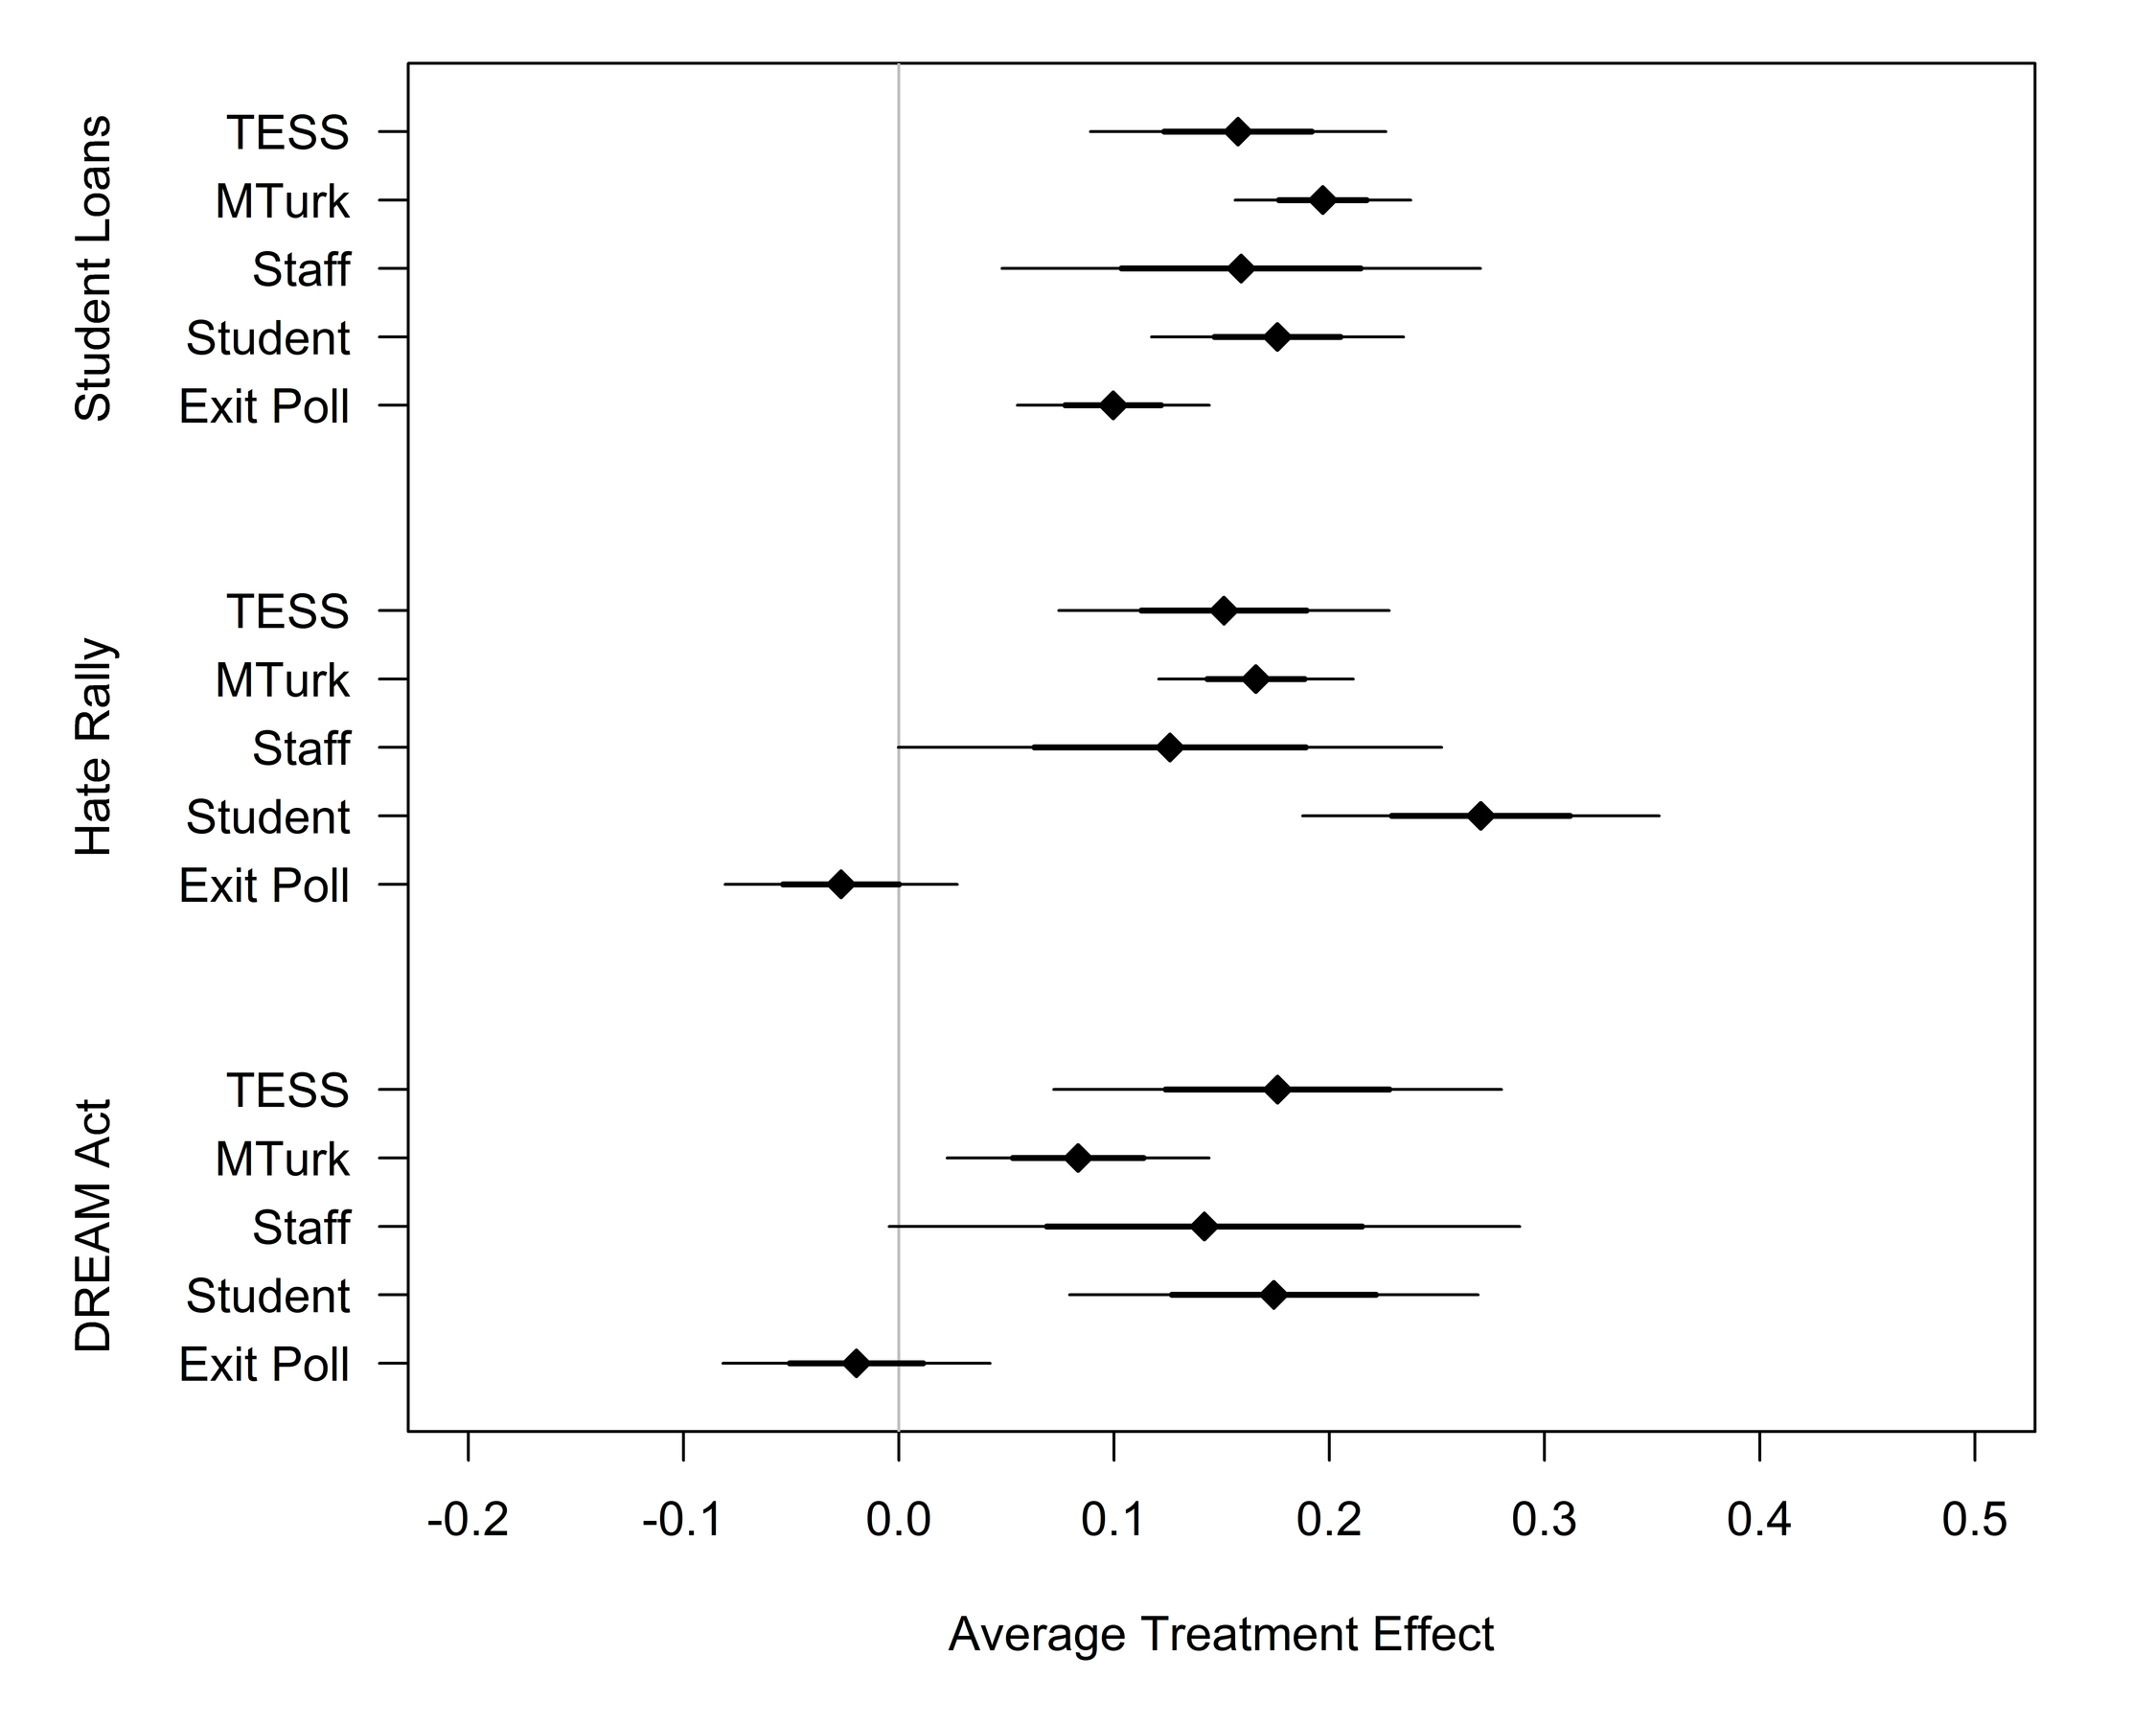
\includegraphics[height=.95\textheight]{images/mullinix3}
\end{center}
}


\frame{
\begin{center}
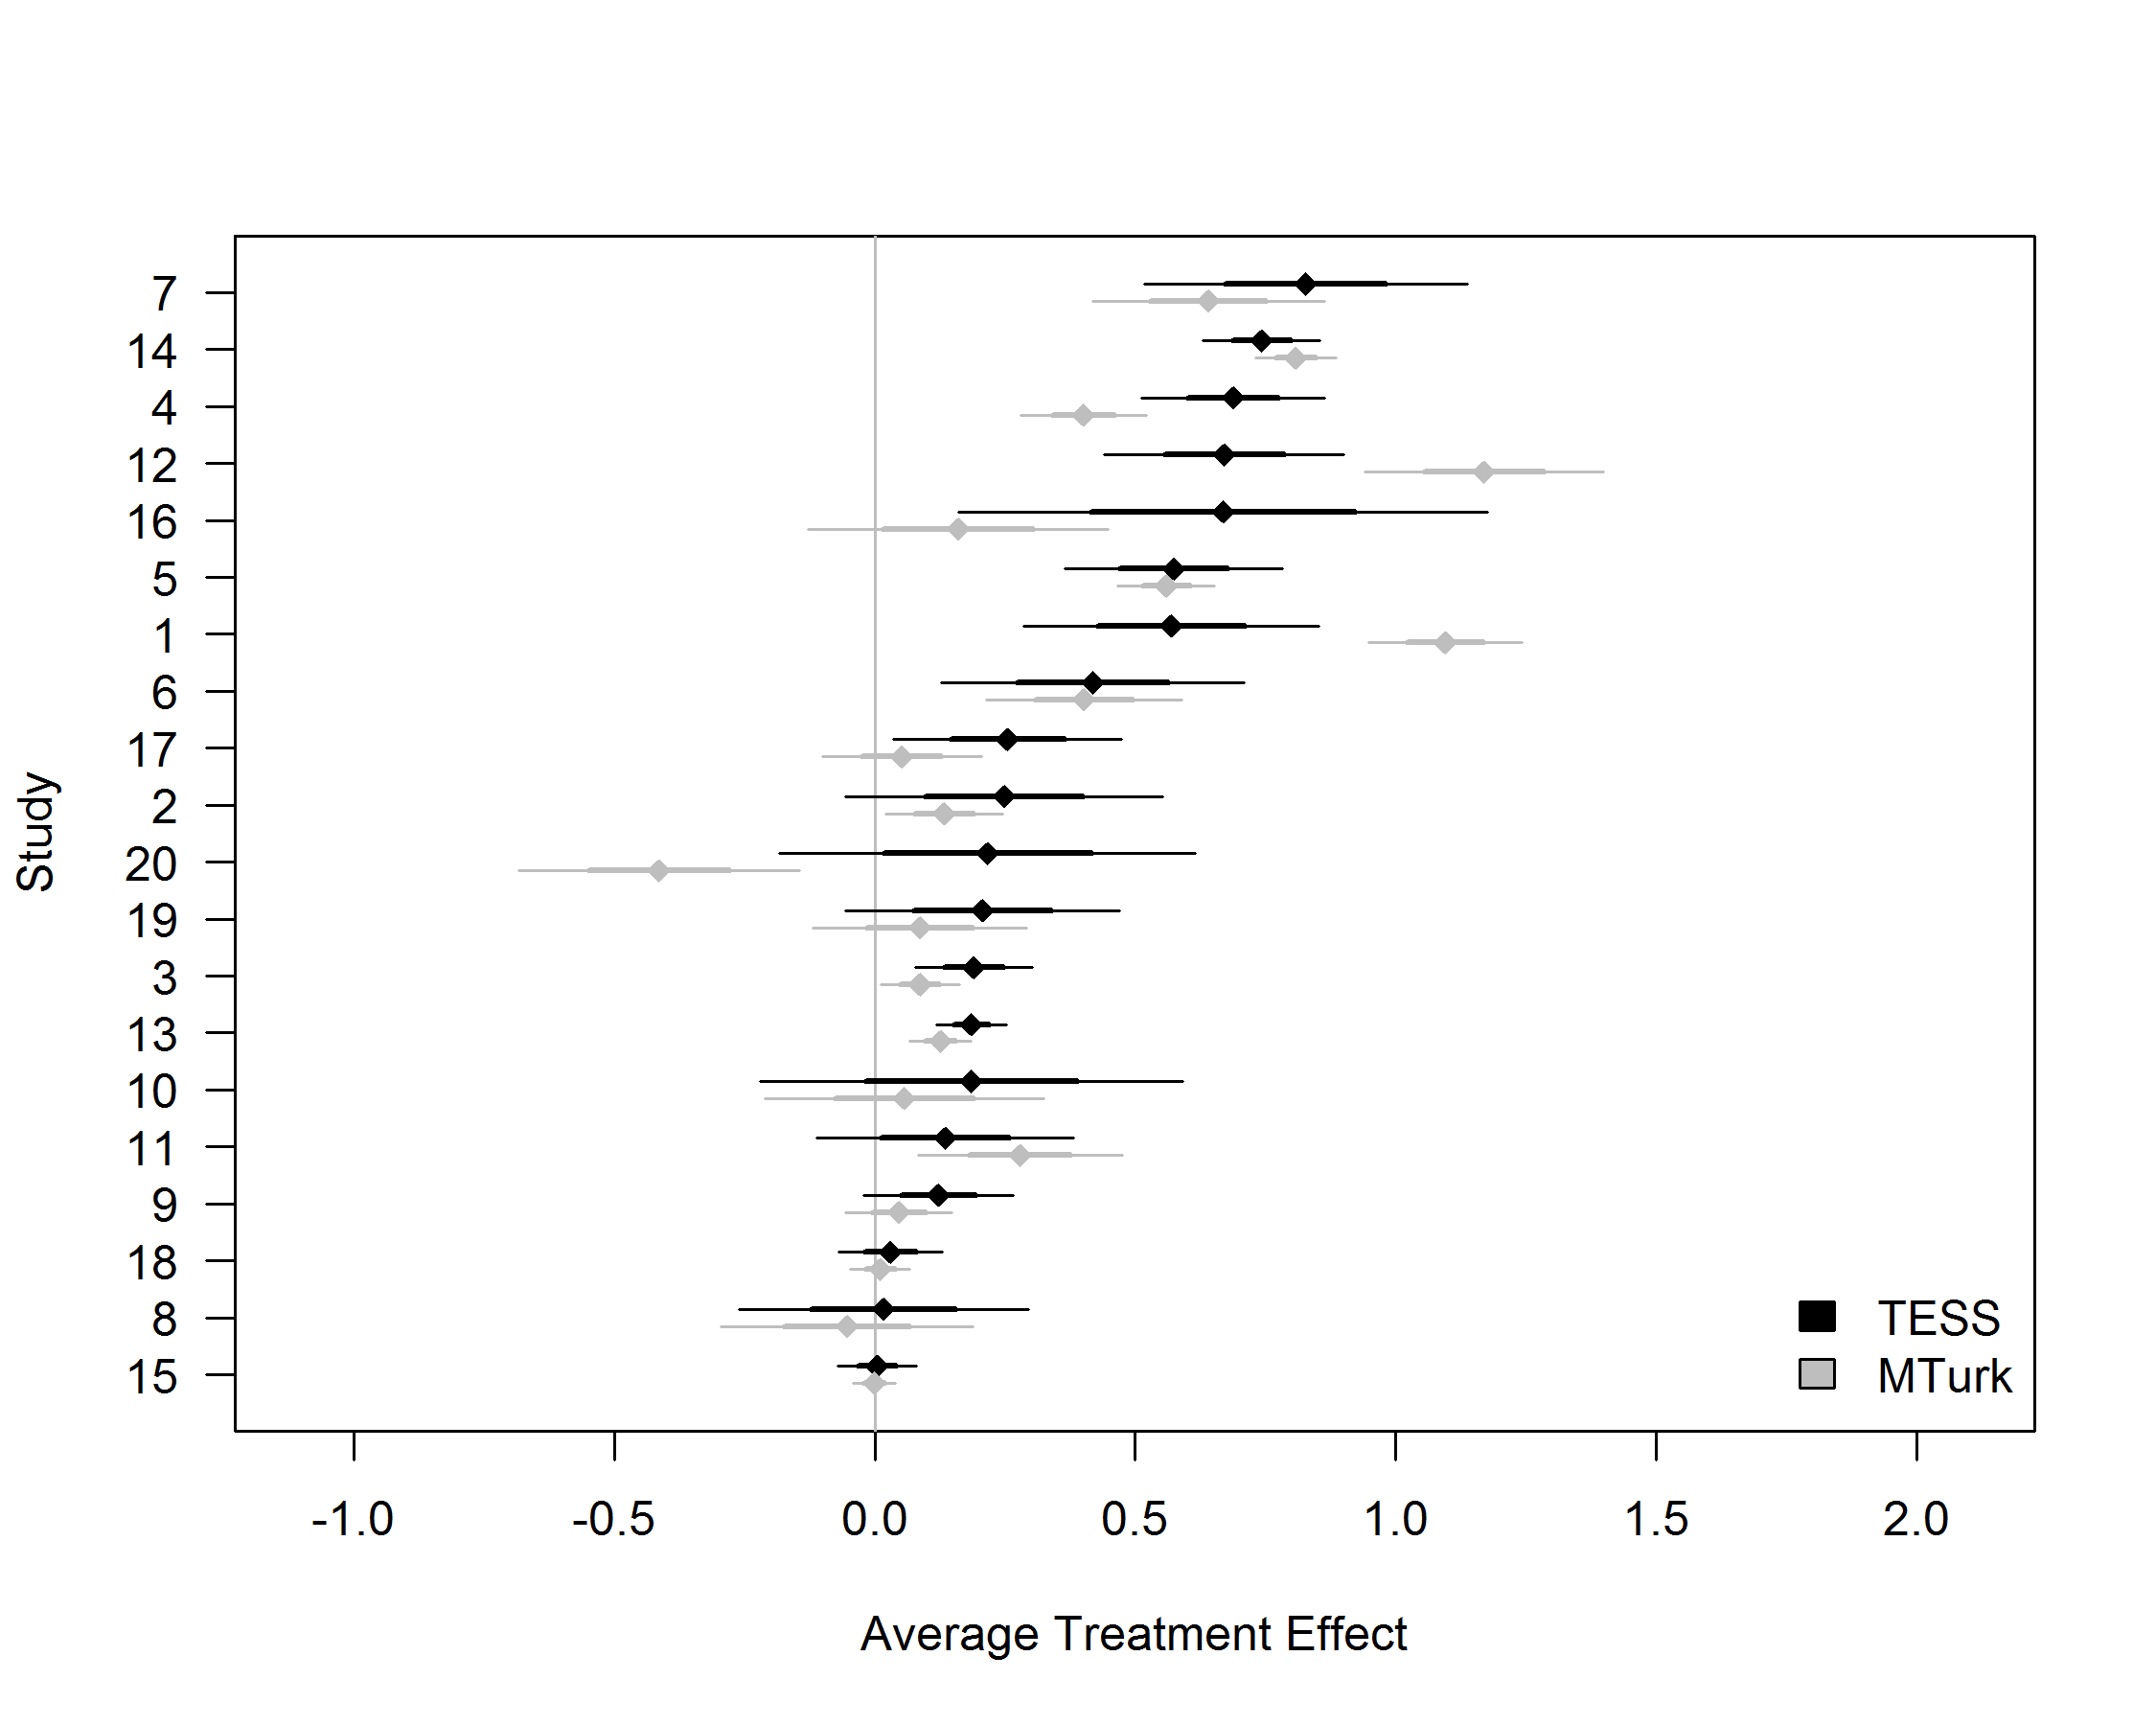
\includegraphics[width=1.1\textheight, trim=0in 0in 0in 0.5in, clip]{images/mullinix1}
\end{center}
}

\againframe<3-4>{myview}

\frame{
\frametitle{Common Differences}
\begin{itemize}\itemsep1em
\item Most common thing to focus on is demographic representativeness
	\begin{itemize}
	\item Sears (1986): ``students aren't real people''
	\item \href{http://www.slate.com/articles/health_and_science/science/2013/05/weird_psychology_social_science_researchers_rely_too_much_on_western_college.html}{Western, educated, industrialized, rich, democratic (WEIRD) psychology participants}
	\end{itemize}
\item<2-> But do those characteristics actually matter?
\end{itemize}
}

\frame{
\frametitle{Common differences}

Shadish, Cook, and Campbell tell us to think about:
	\begin{itemize}
	\item Surface similarities
	\item \textbf<2->{Ruling out irrelevancies}
	\item \textbf<2->{Making discriminations}
	\item Interpolation/extrapolation
	\end{itemize}
}


\frame{
\frametitle{{\normalsize Focus on effect heterogeneity}}

\begin{itemize}
\item<2-> \textbf{Constant effects}: $TE_i$ and $Y_{i0}$ are same for all observations
\item<3-> \textbf{Homogeneous effects}: $TE_i$ is same for all observations
\item<4-> \textbf{Heterogeneous effects}: $TE_i$ is different for all observations
\end{itemize}

}

\frame{
\frametitle{{\normalsize Focus on effect heterogeneity}}

\small

\begin{itemize}\itemsep0.5em
\item Think about and make an evidence-based argument for why you think there are (or are not) heterogeneous effects
\item<2-> If you think there is heterogeneity, then we probably do not care about the SATE anyway
\item<3-> Conditional Average Treatment Effect: $E[Y_{1i} | X = 1, Z=z] - E[Y_{0i} | X = 0, Z=z]$
\end{itemize}
}



\subsection{Model-based}
\frame{\tableofcontents[currentsection, currentsubsection]}

\frame{

\frametitle{Stratification/Blocking}

\small

As soon as we care about heterogeneous effects, it makes sense to stratify and block on factors that might moderate the treatment effect.

\vspace{0.5em}

\onslide<2->{As soon as we identify all sources of heterogeneity, it doesn't matter what sample we use because effects are \textit{by definition} homogeneous within such strata.}

\vspace{0.5em}

\onslide<3->{But, we never know when we've reached that point!}

}



\frame{

If we acknowledge and start thinking about effect heterogeneity, does this mean we can use any convenient group of participants as if they were probability samples?

\vspace{1em}

No. Of course not.
}


% defining your convenience sample
\frame{
	\frametitle{{\normalsize Not All ``Samples'' Are Alike}}
	
	\small
	\begin{itemize}\itemsep0.25em
		\item<1-> Different types:
			\begin{itemize}
				\item<2-> Passive/opt-in/``river sampling''
				\item<3-> Sample of convenience
					\begin{itemize}
					\item Snowball sample
					\item Students
					\item Crowdsourcing
					\end{itemize}
			\end{itemize}
		\item<4-> Differ in numerous ways
			\begin{itemize}
			\item Cost
			\item ``Experience''
			\item Attentiveness
			\item Demographics
			\end{itemize}
	\end{itemize}
}

\frame{
\frametitle{Costs per participant}

From one of my studies:\\

\vspace{1em}

\centering
\begin{tabular}{l r r r}
Sample	& Cost	& n	& Cost/participant\\ \midrule
National	& \$13200	& 593	& \$22.26\\
Exit Poll	& \$3000	& 741	& \$4.05\\
Students	& \$0	& 299	& \$0\\
Staff		& \$1280	& 128	& \$10.00\\
MTurk	& \$550	& 1024	& \$0.54\\
Ads		& \$636	& 80		& \$7.95\\
\bottomrule
\end{tabular}
}

\frame{
\frametitle{Participant Experience}

\small

\begin{itemize}\itemsep0.5em
\item A lot of growing concern about experience
\item Larger literature on ``panel conditioning''
	\begin{itemize}
	\item Inconclusive evidence
	\end{itemize}
\item<3-> Some numbers:
	\begin{itemize}
	\item<3-> MTurk workers are doing 100+ studies per month
	\item<4-> Numbers are the same for YouGov panelists
	\end{itemize}
\end{itemize}

}


\frame{}

% reweighting; pscore methods
\frame{
\frametitle{Reweighting}
\begin{itemize}\itemsep0.5em
\item If effects are heterogeneous, it may be possible to \textit{reweight} unrepresentative data to match a population
\item Any method for this is ``model-based'' (rather than ``design-based'')
\item Not widely used or evaluated (yet)
\item All techniques build on the idea of stratification
\end{itemize}
}


\frame{
	\frametitle{Review of Stratification}
	
	\small
	\begin{enumerate}\itemsep0.25em
		\item Define population
		\item Construct a sampling frame
		\item Identify variables we already know about units in the sampling frame
		\item Stratify sampling frame based on these characteristics
		\item Collect an SRS within each stratum
		\item Aggregate our results
	\end{enumerate}
}


\frame{
	\frametitle{Post-Stratification}
	\begin{itemize}\itemsep0.5em
		\item Used to correct for nonresponse, coverage errors, and sampling errors
		\item<2-> Reweight sample data to match population distributions
			\begin{itemize}
				\item Divide sample and population into strata
				\item Weight units in each stratum so that the weighted sample stratum contains the same proportion of units as the population stratum does
			\end{itemize}
		\item<3-> There are numerous related techniques
	\end{itemize}
}

\frame{
	\frametitle{{\normalsize Post-Stratification: Example}}
	
	\normalsize
	\begin{itemize}\itemsep0.25em
		\item Imagine our sample ends up skewed on immigration status and gender relative to the population\\
	\end{itemize}
	\vspace{0.5em}
	{\small
	\begin{tabular}{lrrlr}
		\hline
		Group             & Pop. & Sample & Rep.                &              Weight \\ \hline
		Native-born, Female    &  .45 &     .5 & \onslide<2->{Over}  & \onslide<3->{0.900} \\
		Native-born, Male      &  .45 &     .4 & \onslide<2->{Under} & \onslide<4->{1.125} \\
		Immigrant, Female &  .05 &    .07 & \onslide<2->{Over}  & \onslide<4->{0.714} \\
		Immigrant, Male   &  .05 &    .03 & \onslide<2->{Under} & \onslide<4->{1.667}\\  \hline
	\end{tabular}
	}
	\begin{itemize}
	\item PS weight is just $w_{ps} = N_l / n_l$
	\end{itemize}
}


\frame{
	\frametitle{Post-Stratification}
	\begin{itemize}\itemsep1em
		\item This is the basis for inference in non-probability samples
		\begin{itemize}
			\item \textit{Demographic} representativeness
		\end{itemize}
		\item Online panels will reweight sample based on age, sex, education, etc.
		\item Purely design-based surveys are increasingly rare
	\end{itemize}
}


\frame{
\frametitle{The Xbox Study}

\begin{center}
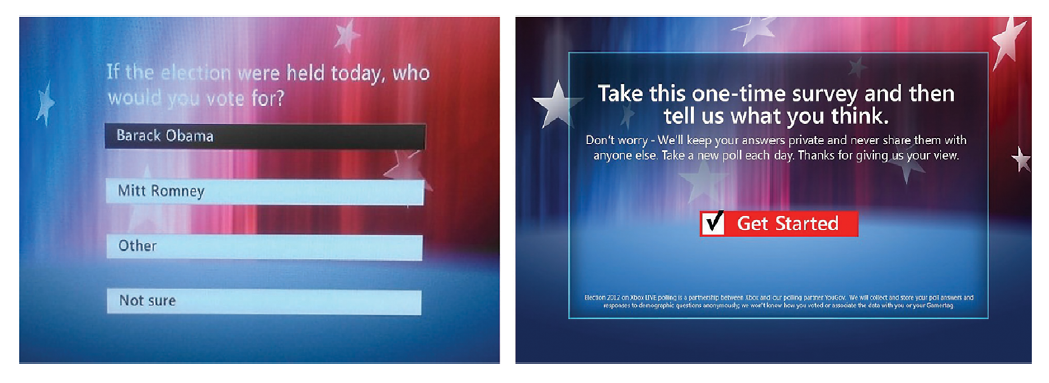
\includegraphics[width=\textwidth]{images/wangetal2}
\end{center}

{\footnotesize Wang et al. 2015. ``Forecasting elections with non-representative polls.'' \textit{International Journal of Forecasting}.\par}

}


\frame{
\frametitle{The Xbox Study}

\begin{center}
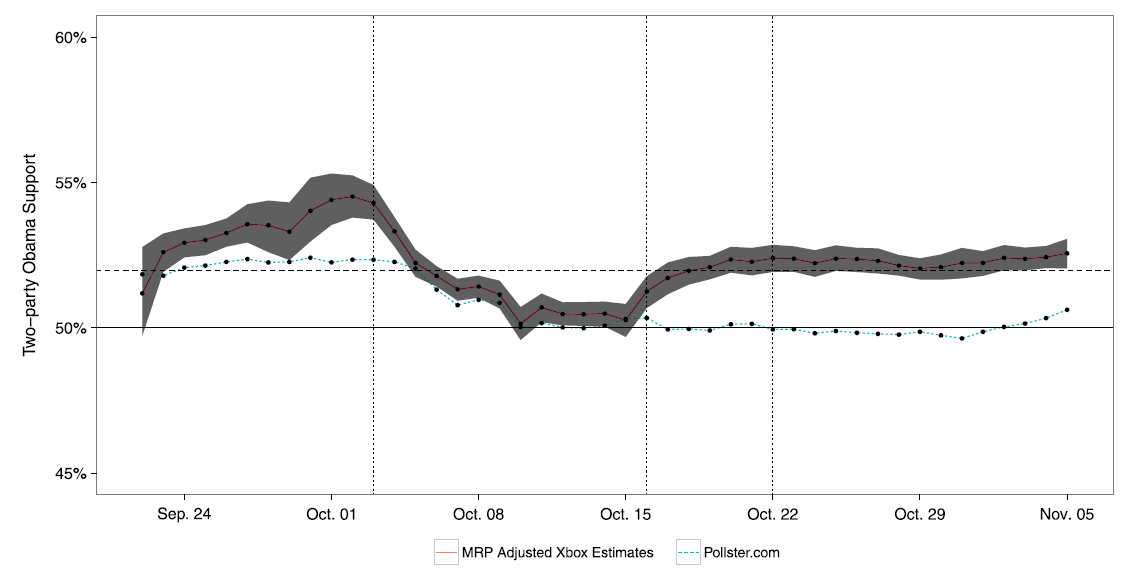
\includegraphics[width=\textwidth]{images/wangetal1}
\end{center}

{\footnotesize Wang et al. 2015. ``Forecasting elections with non-representative polls.'' \textit{International Journal of Forecasting}.\par}

}



\frame{

\vspace{-1.5em}
\begin{center}
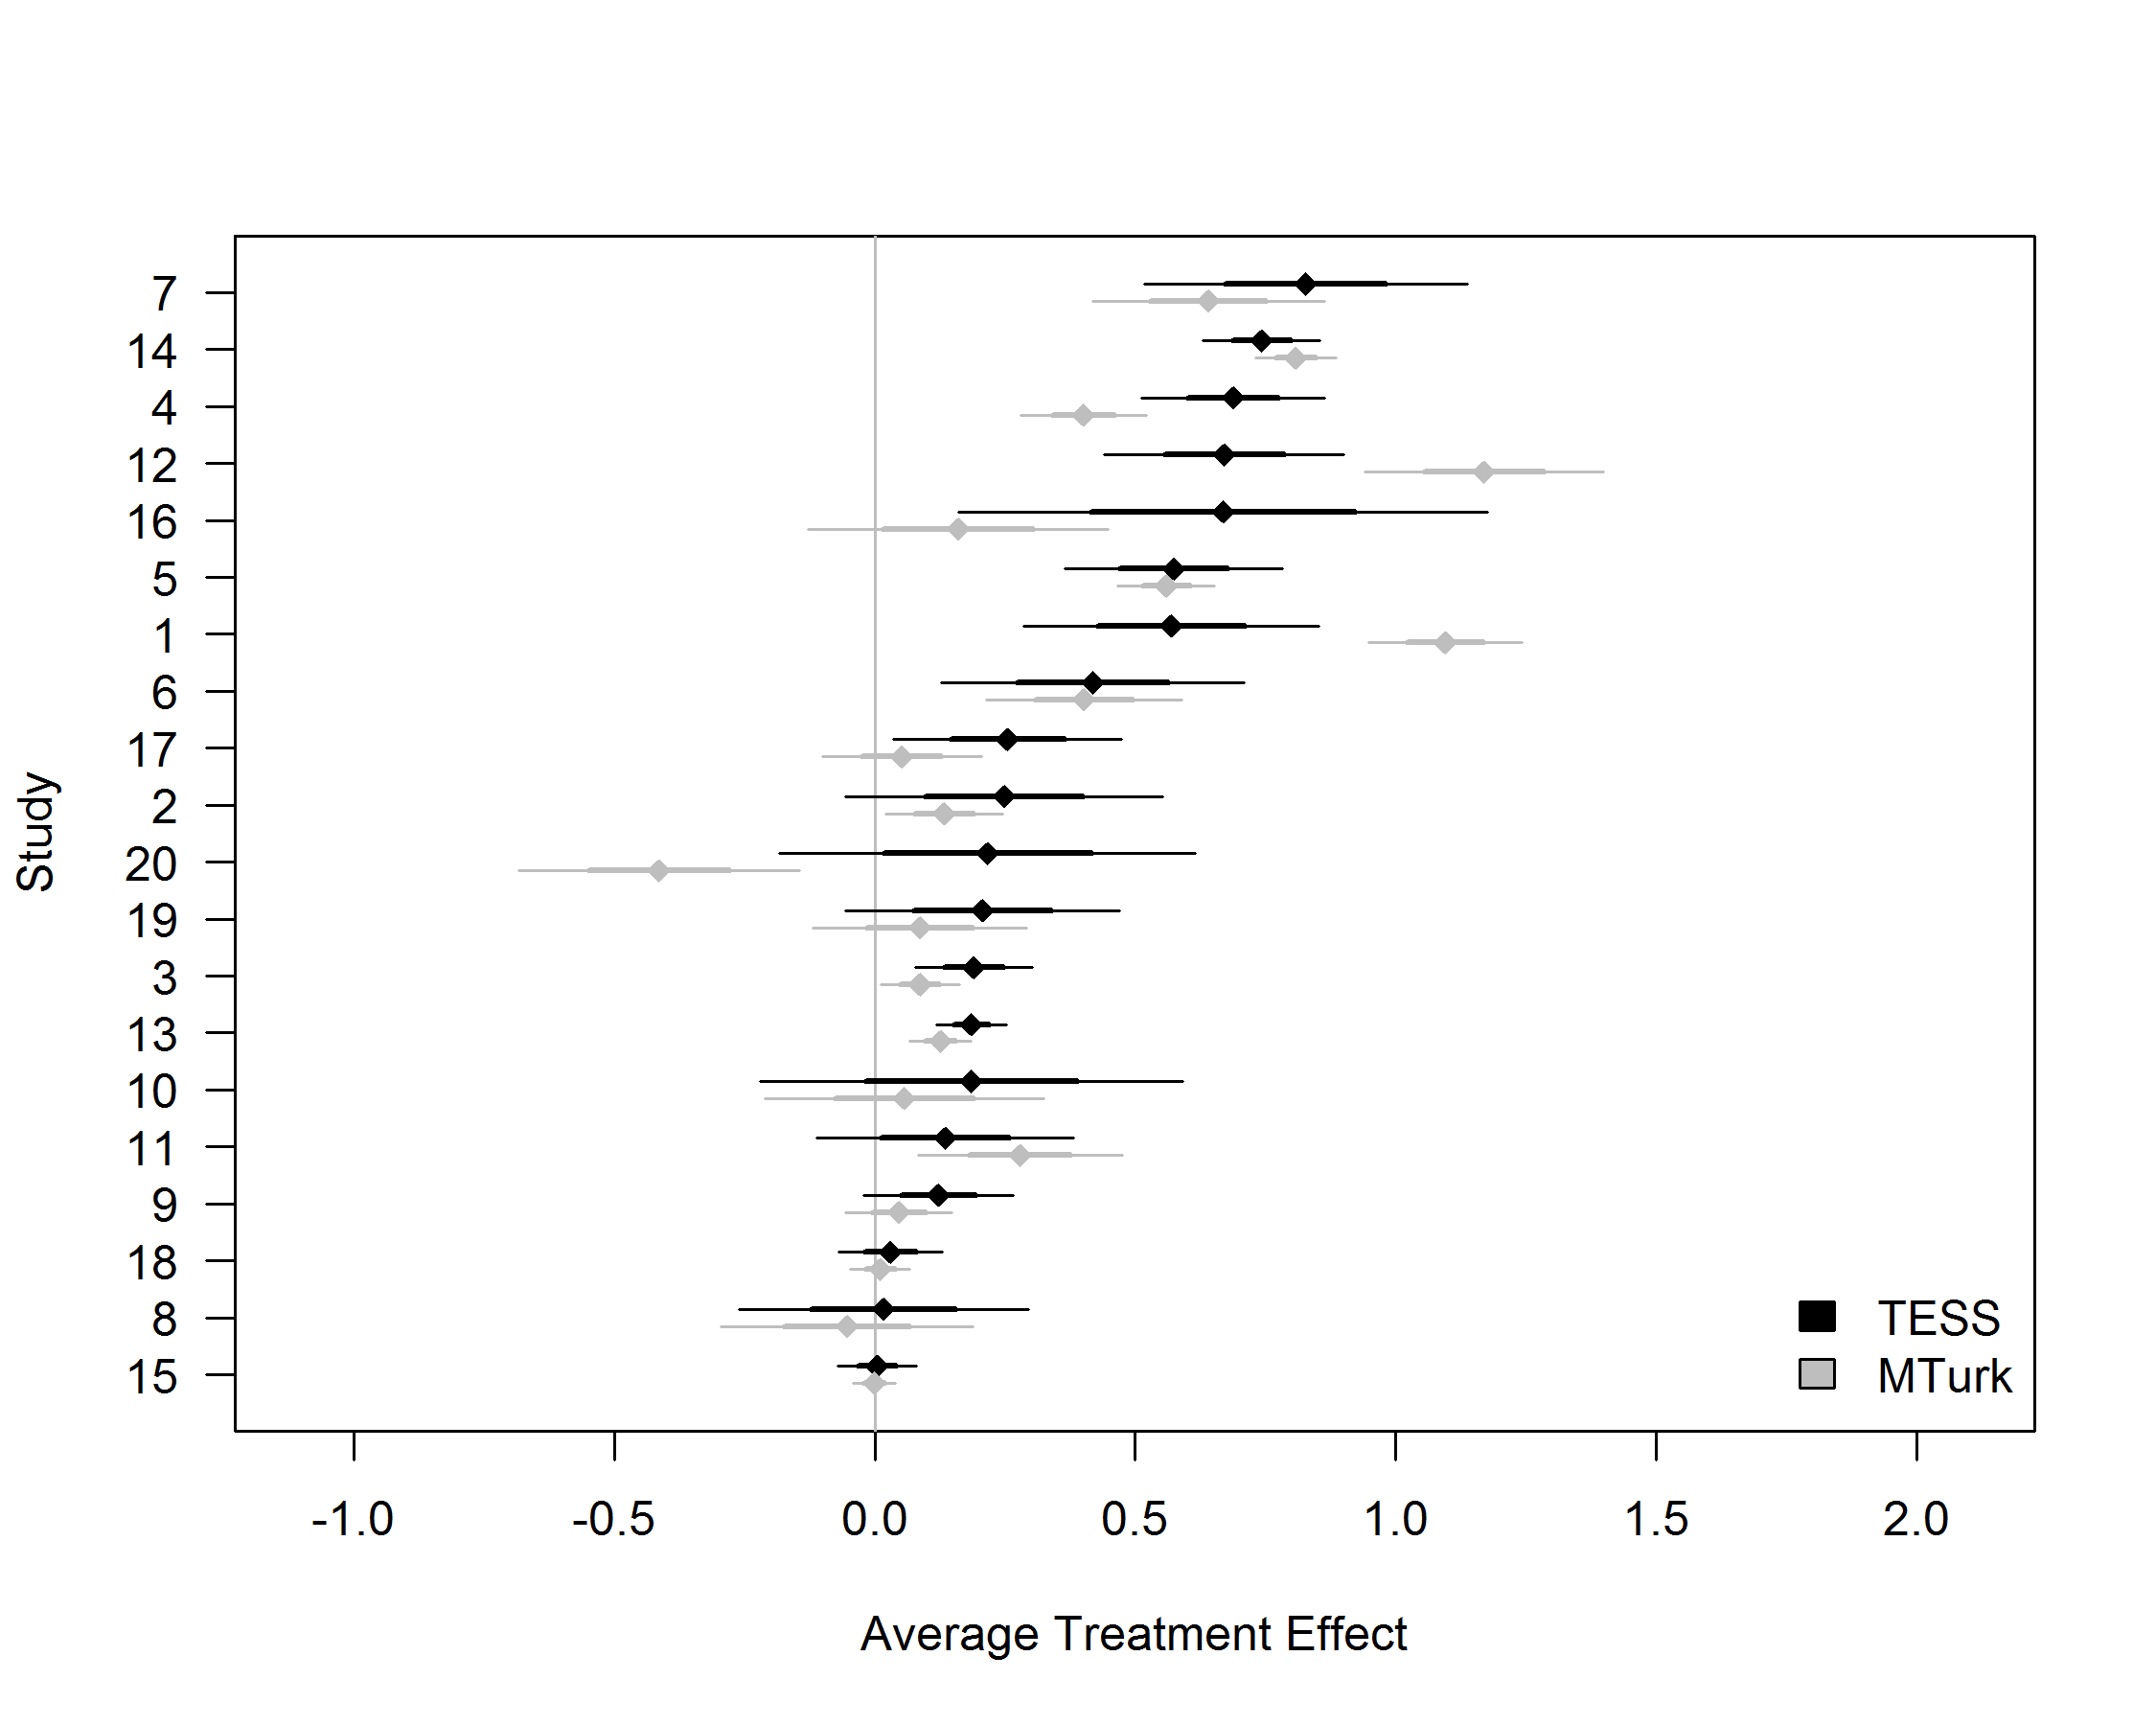
\includegraphics[width=.85\textwidth]{images/mullinix1}
\end{center}
{\footnotesize Mullinix et al. 2015. ``The Generalizability of Survey Experiments.'' \textit{Journal of Experimental Political Science}.\par}
}

\frame{
\vspace{-1em}
\begin{center}
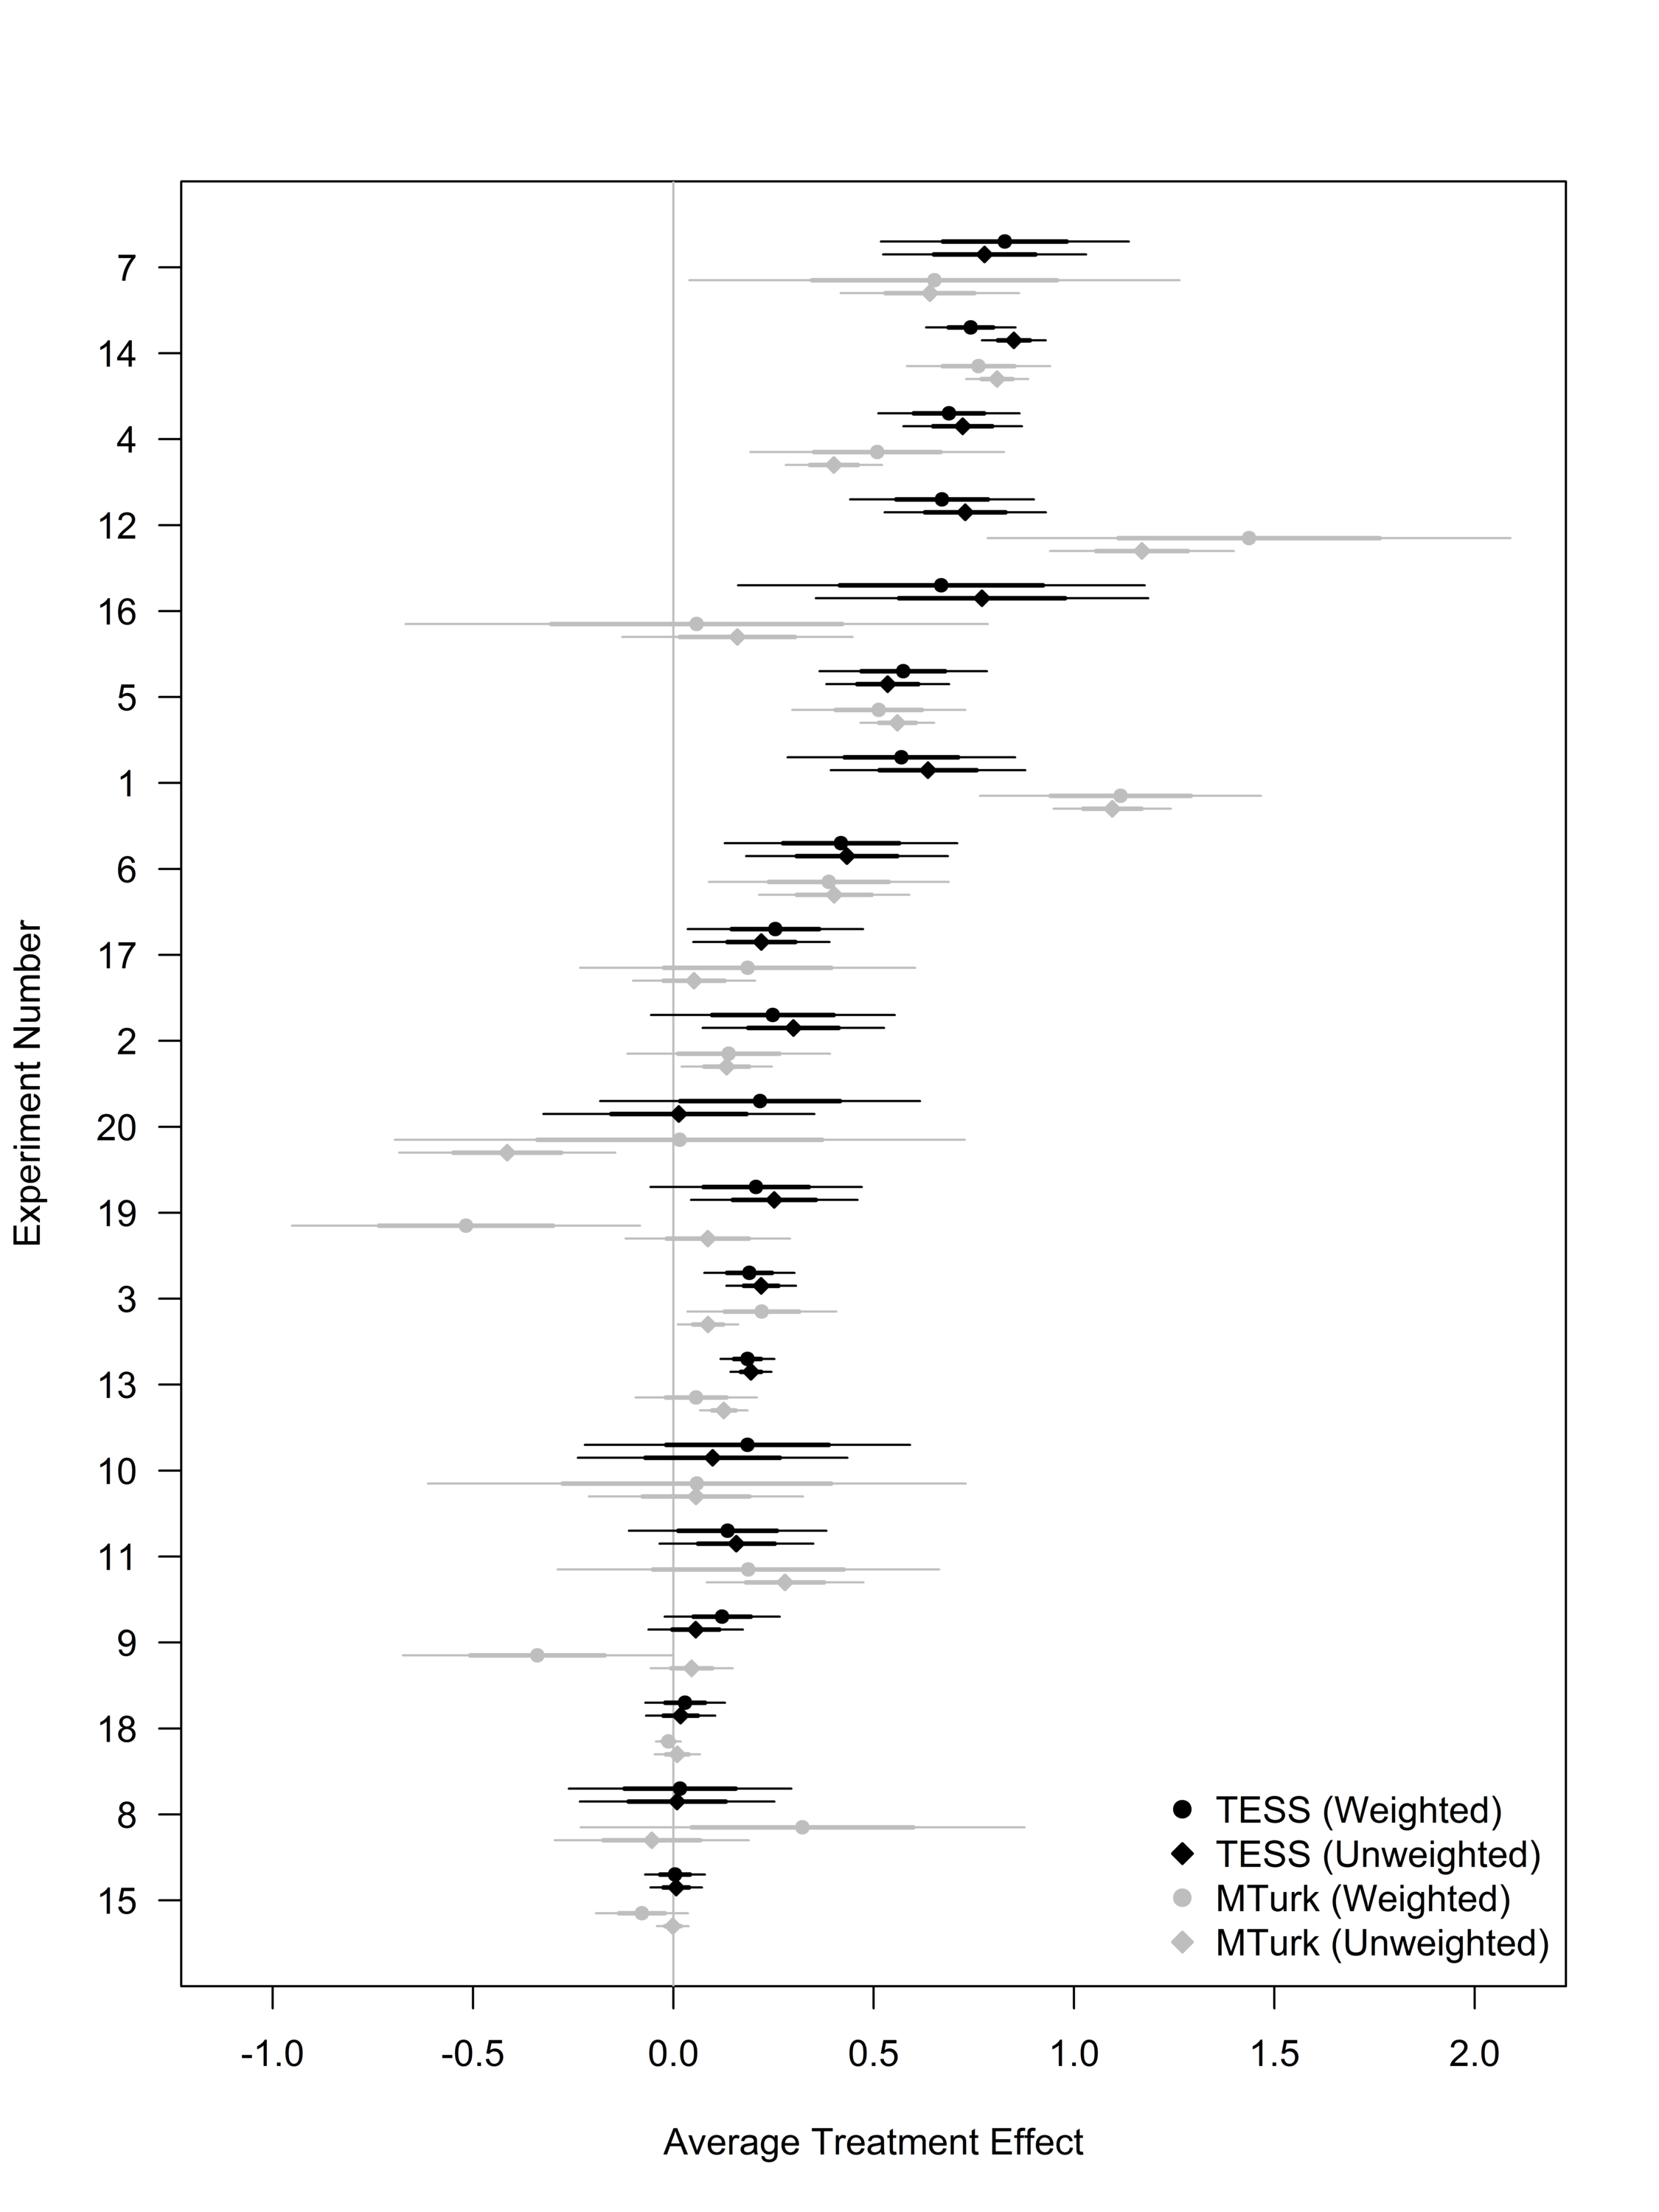
\includegraphics[width=.8\textheight]{images/mullinix2}
\end{center}
}



\frame{
\frametitle{{\normalsize Propensity Score Approach}}

\small

\begin{enumerate}\itemsep-0.2em
\item Define a target population 
\item Estimate a propensity score model
	\begin{itemize}\footnotesize
	\item Pool experimental samples and target population units
	\item Predict membership of all target and sample units in the experimental sample
	\end{itemize}
\item Using fitted logits, divide population \& sample into strata
\item Estimate stratum-specific ATE
\item Calculate weighted average of stratum-level estimates
\end{enumerate}
}


\frame{
\frametitle{{\normalsize Propensity Score Approach}}

Target population average treatment effect:
\begin{equation}
\sum_{v=1}^{5} p(v)T(v)
\end{equation}
where $p(v)$ is the proportion of the target population in a given stratum, $v$, and $T(v)$ is the estimated effect from stratum $v$ of the experimental sample
}


\frame{
\frametitle{Propensity Score Approach}

Effect variance:
\begin{equation}
\sum_{v=1}^{5} p(v)^2 V(v),
\end{equation}
where $V(v)$ is the variance of the estimated experimental sample effect for stratum $v$
}



\frame{
\frametitle{Propensity Score Subclassification Estimator}
\begin{columns}
\column{\dimexpr\paperwidth-12pt}
\scriptsize
\begin{tabular}{rrrrrrrrr} \toprule
& \multicolumn{2}{c}{Weights} & \multicolumn{6}{c}{Estimates}\\
Stratum & Nat'l & Sample & Loan & DREAM 1 & DREAM 2 & Rally \\% & Rally (Distant) & Rally (Local) \\ 
  \midrule
  1 & 0.20 & 0.83 & 0.94 (0.08) & 0.06 (0.11) & -0.22 (0.12) & 0.74 (0.10) \\% & 0.77 (0.15) & 0.72 (0.15) \\ 
  2 & 0.20 & 0.11 & 0.99 (0.26) & 0.22 (0.37) & -0.28 (0.36) & 0.77 (0.29) \\% & 0.85 (0.39) & 0.70 (0.42) \\ 
  3 & 0.20 & 0.04 & 1.28 (0.43) & -0.61 (0.58) & -1.76 (0.54) & 1.00 (0.45) \\% & 0.75 (0.64) & 1.26 (0.64) \\ 
  4 & 0.20 & 0.01 & 1.99 (0.73) & 0.29 (1.12) & 0.56 (0.89) & 1.44 (0.79) \\% & 3.13 (1.95) & 1.54 (0.63) \\ 
  5 & 0.20 & 0.00 &  &  &  &  &  &  \\ \midrule
  Sample & - & - & 1.04 (0.30) & -0.01 (0.44) & -0.34 (0.38) & 0.79 (0.33) \\% & 1.05 (0.60) & 0.86 (0.37) \\ 
  Nat'l & - & - & 1.14 (0.18) & 0.02 (0.22) & -0.94 (0.23) & 0.94 (0.19) \\% & 1.01 (0.26) & 0.93 (0.27) \\ 
   \bottomrule
\end{tabular}
\end{columns}
}


\frame{
\frametitle{{\normalsize So does reweighting solve everything forever?}}

\begin{itemize}\itemsep0.25em
\item<2-> Need well-defined target population
	\begin{itemize}
	\item and detailed covariate data
	\item and large stratum sizes
	\end{itemize}
\item<3-> Purely model-based, so only as good as the model
	\begin{itemize}
	\item What unobservables might there be?
	\item What reweighting might worse bias?
	\end{itemize}
\item<4-> Non-coverage is a potential problem
\item<5-> Not well-tested on experimental data
\end{itemize}

}



\questions

\section[SUTO]{Other Notions of External Validity}
\frame{\tableofcontents[currentsection]}


\frame{
\frametitle{SUTO Framework}
\begin{itemize}\itemsep0.5em
\item Cronbach (1986) talks about generalizability in terms of UTO
\item Shadish, Cook, and Campbell (2001) speak similarly of:
	\begin{itemize}
	\item \textbf{S}ettings
	\item \textbf{U}nits
	\item \textbf{T}reatments
	\item \textbf{O}utcomes
	\end{itemize}
\item External validity depends on all of these
\end{itemize}
}


\frame{
\begin{columns}[t]
\begin{column}{0.5\textwidth}
	\begin{block}{Population}
		\begin{itemize}
		\item Setting
		\item Units
		\item Treatments
		\item Outcomes
		\end{itemize}
	\end{block}
\end{column}
\begin{column}{0.5\textwidth}
	\begin{block}{Your Study}
		\begin{itemize}
		\item Setting
		\item Units
		\item Treatments
		\item Outcomes
		\end{itemize}
	\end{block}
\end{column}
\end{columns}

\vspace{0.5em}

\small

\only<2->{In your study, how do these correspond?\\}
\only<3->{\hspace{5.7em} how do these differ?\\}
\only<4->{\hspace{5.7em} do these differences matter?\\}

}


\frame{

\frametitle{Pretreatment Dynamics}

``If the experiment explores a communication that regularly occurs in `reality,' then reactions in the experiment might be contaminated by those `regular' occurrences prior to the experiment.'' \footnote{p.875 from Druckman \& Leeper. 2012. ``Learning More from Political Communication Experiments: Pretreatment and Its Effects.'' \textit{American Journal of Political Science} 56(4): 875--896.}

}

\frame{

\frametitle{Pretreatment Dynamics}

\small
\begin{itemize}
\item Pretreatment is a feature of an experimental setting, treatment, and sample, wherein the effect of the treatment has already occurred\footnote{Or, units having already been treated are otherwise affected differently.}
\item<2-> Consequences:
	\begin{itemize}\footnotesize
	\item Biased effect estimates
	\end{itemize}
\item<3-> Mitigation:
	\begin{itemize}\footnotesize
	\item Measure pretreatment
	\item Avoid ``pretreated'' treatments or contexts
	\item Study units not already treated
	\item Theorize repeated effects
	\end{itemize}
\end{itemize}

}

\frame{

\frametitle{{\normalsize Behavioral Outcomes}}

\small

\begin{itemize}
\item Survey experiments can rarely measure \textit{behavior}, only \textit{attitudes} or \textit{behavioral intentions}
\item Consequences:
	\begin{itemize}\footnotesize
	\item Lack of external validity
	\item Overestimates (typically) of behavioral intentions or past behavior
	\end{itemize}
\item Mitigation:
	\begin{itemize}\footnotesize
	\item Acknowledge limitations
	\item Incentivized surveys or games
	\item Small behaviors
	\end{itemize}
\end{itemize}

}


\questions


\frame{

\frametitle{Small Group Activity!}

In groups of 4--5, consider examples from TESS, Tuesday's lecture, or your own experiences. Discuss:
\begin{itemize}\small
\item What was the researcher's question? How did they test it experimentally?
\item Thinking of SUTO, in what ways is the study externally valid? In what ways is it not externally valid?
\end{itemize}

Take about 7--8 minutes.

}


\questions

\frame{

\frametitle{Homework!}

None! Enjoy your Wednesday!

}


\appendix
\frame{}

\end{document}
